\chapter{Phonetic Accommodation}
\label{chap:phonetic_convergence}

\lettrine{I}{n} this chapter, the concept of accommodation is introduced.
Types of linguistic changes and they way similar terms are used in this work are explained as well.
Finally, a survey of works on phonetic convergence in \acl{hci} lays the ground to the novel work presented in this work.

\pagebreak

\section{\Acl{cat}}
\label{sec:communication_accommodation_theory}

Communication is an fundamental part of life.
In addition to offering a means to exchange information and express emotions and desires, it also exhibits salient social category memberships
Human communication is a complex concept concealing many facets and sub-processes within it.
This Complexity stems from two main aspects:
First, each individual is unique and communicates differently -- in general as well as in specific interactions -- based on inherent traits, emotional state, personal preferences, situational circumstances, and more.
Moreover, an interlocutor may belong to a certain group or represent one (e.g., a social group or an organization), which may also influence the nature of the exchange.
Secondly, some form of communications, in particular face-to-face, harness combinations of modalities.
This results in a large amount of data one needs to process in real-time to obtain maximal efficiency.
Furthermore, despite common social conventions, not every person perceives and processes this information the same way, which requires from all interlocutors to be attentive as they how they comprehend the others and are being understood by them.
Therefore, each exchange is unique and shaped by various personal and environmental factors (more in  \cref{subsubsec:dialogue_is_hard}).
To cope with such highly variable dynamics, people must have some way to know -- whether unconsciously, intuitively, or deliberately -- how to adjust their communicative behavior.

\Acf{cat} is a theoretical framework of communication introduced by \citet{Giles1973mobility, Giles1991CAT, Giles2007CAT}, which aims to explain the personal and social motivations in verbal and non-verbal human communication.
A core motivation in \ac{cat} is \emph{social distance}.
To reduce social distance, a speaker may converge to the conversation partner(s), whereas divergence would lead to increase in social distance.
When and how social distance should be altered depends on the social class of the speakers, their formal role and personal goals in the interaction, etc.
Particularly, these changes occur with respect to how the other conversation partners speak, from overall psychological, social and linguistic behaviors to specific features (like those in \cref{subsec:linguistic_accommodation}).
For example, different communication styles would probably be utilized when speaking to a childhood friend, a colleague, or a company's executive.
In each of these situations, it is likely that the speakers would use different language registers (e.g., slang words and politeness) in attempt to fit into the social groups or become socially closer.
Another example is the use of \enquote{elder language} when talking to old people (e.g., talking more slowly, extended use of hand gestures, etc.), to make it easier for them to understand the speaker.
Such adjustments can be, to some extent, conscious, but often occur automatically.
Ideally, both speakers find their comfort zone during the conversation.
However, there exist the notion of over-accommodation, which is usually a result of a very conscious speaker that intentionally exploits this phenomenon.
If realized by a conversation partner, this might be perceived as pretentious or fake behavior and even mockery.
Similarly, accommodation can serve a speaker with audience design when talking to larger group of people.
\todo{if need a reference, find something on \url{https://en.wikipedia.org/wiki/Audience_design}}
The adjustments may be reflected simultaneously in different modalities, like hand gestures, body posture, facial expression, eye gaze, lexical choices, and speech.
\todo{find one reference for each non-linguistic example}
This work concentrates on linguistic aspects, and speech in particular.
Detailed examples of linguistic accommodation are described in \cref{subsec:linguistic_accommodation}.
While \ac{cat} advocates these changes, it is worth noticing that there are other further frameworks that explain them.
For instance, the Interactive Alignment Model \citep{Pickering2004behavioral, Pickering2013integrated} offers a model where adjustments in communicative behavior are described as \emph{alignment} as opposed to \emph{accommodation}, hinting that the process is rather one-sided and uni-directional (see \cref{tab:variation_types}).
Despite this difference and others, all these frameworks describe a process where the similarity between interlocutors increases or decrease with respect to certain features over the course their communication.
\Cref{subsec:variation_types} sheds more light on the difference between the different terms used to describe this process and how they are used in the literature.

\todo[inline]{find an example for each non-linguistic modality mentioned (put in parantheses like "(e.g., moving the hands the same way (CITE))}

\subsection{Linguistic accommodation}
\label{subsec:linguistic_accommodation}

Accommodation occurs on various linguistic levels in \ac{hhi}.
Relative salient changes may occur on the lexical level when one interlocutor shifts his lexical choices to match those of another.
This is more likely to happen when a lexical entity has multiple commonly used alternatives, like synonyms or different names.
\citet{Jucks2008lexical} shows how healthcare experts try to match their wording to patients in written inquiries.
In another experiment, \citet{Friedberg2012lexical} found increasing lexical similarity over the course of spoken discussion among students groups with better performances.
\citet{Racz2020morphological} even extended the analysis to morphological forms, suggesting that morphological convergence occurs and creates generalizations in memory in real-time.
over these instances.
Another examples of lexical convergence have also been found in \ac{hci} when looking for information \citep{Lopes2013lexical} and when playing \citep{Bergqvist2020nontrivial} (and see \cref{subsec:previous_work}).
In all these experiments, it was shown that lexical convergence had a positive effect on the performance of the speakers.

The focus in this work is on accommodation occurring in speech-related features, i.e., \emph{vocal accommodation}.
A core difference between lexical and vocal accommodation is the mechanism for defining two instances as the same.
For example, the word \enquote{window} is written the same way regardless of who writes it (this is especially true if the word typed), which makes it easy to associate tokens with the same type.
However, vocal features are strongly dependent on the speaker.
The signal representing a word would be different depending on the speaker's physiological properties (like vocal tract size), natural speaking rate, voice intensity, intonations, and many more.
Moreover, it is very unlikely that even the same speaker would pronounce the same word in the same manner.
This is especially true in conversation taking place in different setting and environments, but also for two successive utterances in the same conversation.
Additionally, the relative differences, e.g., in vowel quality or speaking rate, also differ from one person to another, which entails that more evidence might be needed for a perceivable target for accommodation to emerge.
An exception to these differences could be categorical phonetic differences, where each category may be perceived as a separate entity (similarly to the lexical case), making it easier to define the target (and see \cref{subsec:target_features_HCIConv,subsec:speech_manipulation}).
This great variety in spoken language makes the accommodation process somewhat more complex, as the targets might not always be well-defined and static.
%(comparing with a lexical entity that would always be recognized as the same).

Vocal accommodation has been found in both segmental \citep{Pardo2010conversational, Smith2007prosodic} and suprasegmental \citep{Walker2015repeat, Shockley2004imitation} phonetic features and
both in conversational \citep{Pardo2006phonetic, Lewandowski2012talent, Weise2018looking} and non-conversational \citep{Babel2014novelty, Shockley2004imitation} scenarios.
There is evidence for it being both an internal mechanism \citep{Pickering2004behavioral} and socially motivated \citep{Kim2011phonetic, Giles1991CAT}.
For instance, phonetic convergence \citep{Giles1973mobility} or divergence \citep{Bourhis1977distinctiveness} is triggered with decreasing or increasing social distance between interlocutors, respectively.
\Citet{Baumann2020how} even shows that feedback given by conversation partners can influence the convergence process.
As demonstrated by \citet{Pardo2013measuring}, vocal accommodation can occur with respect to numerous phonetic features.
\citet{Aubanel2020speaking} found that speakers accurately and consistently converge to each other's pitch (\ac{f0}) in scripted read-aloud dyadic conversation on a turn-by-turn basis.
This shows the ability to track changing \ac{f0} both in perception and production.
The study conducted in \citet{Babel2012role} supports the importance of \ac{f0} in convergence effects by showing that filtering out the \ac{f0} frequencies in the signals the participants hear leads to reduced convergence.
\citet{Schweitzer2017visibility} shows that convergence effects are stronger when conversation partners can speak but not see each other, and divergence occurs more when they can also see each other while talking.
Moreover, the effects were stronger depending on the degree of likability between them.
This shows that accommodation can be influenced by other, no necessarily linguistic factors of the conversation.
According to \citet{Lehnert2020relationship}, language skill level and greater \ac{f0} expressiveness also influence the degree of convergence.
Accommodation effects were also found in intensity.
In an experiment where participants heard an interviewer in different levels of vocal intensity, \citet{Natale1975convergence} shows that their intensity was generally changed accordingly.
In a second experiment, the degree of intensity convergence could be predicted by a social desirability test, which stands in line with the finding of \ac{f0} accommodation.
A third studied feature is speaking rate (and sometimes \acf{ar}).
In an exemplar-theoretic view in mind, \citet{Schweitzer2016exemplar} investigated how syllable frequency influences the degree of change.
Evidently, stronger effects were found in more frequent syllables, which supports this view.
Relatedly, \citet{Edlund2009pause, Xiao2015analyzing, Cohen2017converging} introduce ways to measure temporal prosodic changes, like pauses, in conversation, which affect the speaking rate.
\citet{Levitan2011measuring, Local2007phonetic} found convergence effects in all these three features (and others) in collaborative games and every-day scenarios.
Such wide variety of evidence suggest that, even in the vocal modality alone, accommodation is reflected in various ways in \acp{hhi}.
These features are investigated in this work in both \ac{hhi} (\cref{chap:conv_analysis}) and \ac{hci} (\cref{chap:speech_variations_in_hhci}) contexts.
In addition to these, other factors and phonetic features were investigated for accommodation, such as voice quality \citep{Borrie2017conversational}, voice onset time \citep{Nielsen2011specificity} and other timing-related phenomena \citep{Putman1984conception}, second language proficiency \citep{Law2020convergence}, interlocutors' sex \citep{Levitan2012acoustic, Bailly2014assessing}, perceived attractiveness \citep{Michalsky2017pitch}, word frequency \citep{Nenkova2008high}, and more.
Further methods and ways to measure accommodation in \ac{hhi} can be found in \citet{Lewandowski2019phonetic, DeLooze2014investigating}.

\subsection{Limitations of \acl{did} measures}
\label{subsec:limitations_of_did}

\todo[inline]{consider changing the title of this subsec to something more general like "limitations and aspects" (also to be able to write more general things}

\todo[inline]{a few sentences (where?) that *two* aspects are missed by DiD -- temporal and directionality}

%\subsection{Conversation-level accommodation behavior}
%\label{subsec:conversation-level_accommodation_behavior}

Conversations are complex processes that require some expertise and some quantitative analysis to detect and isolate specific patterns in them.
All the more so, since effects may have long, non-linear relations.
A behavior is a complex collection of conducts of a person (and any organism, system, or artificial entity), particularly those towards a certain environment.
The realization of one's behavior over the course of a conversation can communicate information regarding one's state and goals, especially with this deviates from the individual's expected behavior.
The behavior leads to reactions to environmental input and can be modified due to reinforcements from the environment or self-directed motives.
These modifications can occur over time quickly or slowly, consciously or unconsciously, and to greater or lesser extends, which makes them dynamic and thus cannot be defined discretely.
All the above is true also for vocal behaviors, which are expressed in spoken interactions.
Specifically, vocal accommodation reflects dynamic changes during conversation that can be affected by the external speech input of other interlocutors.
It can therefore be beneficial to \textbf{move away from value comparisons in favor of behavior descriptors} to depict an interaction.
This is done by analyzing spoken interactions as entire events with a continuous temporal dimensions as opposed to a comparison between some discrete points in time.
Examining the whole conversation can help, for example, to determine who was leading the changes or when more accommodation occurred.
In this work, such analyses were utilized in \cref{chap:conv_analysis} to determine the leading speaker in each conversation and in \cref{chap:speech_variations_in_hhci} to expose the ongoing changes in the human speaker's productions.

The way speakers accommodate to each other is very unlikely to be linear from beginning to end and can change throughout the conversation.
Therefore, comparing the differences between two discrete, distant points in time might miss or oversimplify some dynamics that occurred between them.
Moreover, comparisons like that must inherently take the view of one speaker instead of looking at the conversation as a complete entity.
Quantitative analyses often leave accommodation hidden or overly-simplified if analyzing a conversation on turn-by-turn basis or by splitting it arbitrarily into two or more parts (often equally-long, non-overlapping time intervals) and directly comparing them using raw values as in \citet{Heldner2010pitch, Rahimi2018weighting, Ibrahim2019fundamental}.
\citet[][p.~15]{DeLooze2014investigating} points out that in these cases it is assumed that accommodation is a strictly local phenomenon where a speaker's utterances is linked exclusively to the other interlocutor's immediate preceding utterance.
Such analyses result in a linear, static representation of the conversation's evolution, from which generalized conclusion are hard to draw.
They might even be inaccurate or misleading, especially when both speakers change their output over time, as demonstrated by \citet{CohenPriva2019limitations}.
That work specifically refer to \ac{did} measurements, where pairs of two discrete points in time are compared to measure accommodation between speakers using the following distance formula\footnote{Note that this way of measuring \ac{did} is commutative and therefore doesn't measure the changes from the view of a specific speaker \citep[unlike,~e.g.,][p.~3]{CohenPriva2019limitations}.}
%
\begin{equation}
	\label{eq:did}
	DiD_{\vec{i},\vec{s}} \coloneqq \sqrt{(\vec{i}_{t + 1}^n - \vec{s}_{t + 1}^n)^2 + (\vec{i}_t^n - \vec{s}_t^n)^2} \equiv \lVert \vec{i} - \vec{s} \rVert_n.
\end{equation}
\eqname{\Acl{did} measure (simplified)}
\noindent
%
\cref{fig:accommodation_types} shows the interaction between two speakers' productions in a hypothetical conversation.
By merely looking at the plot, it is clear that the two speakers do not sustain the same behavior throughout the conversation.
For example, between marks A and B the orange speaker's values go remarkably downwards (though not linearly), while the green speaker remains roughly stable -- i.e., \emph{divergence} (although this can also be seen as an independent changes).
Subsequently, between B and C the distance is generally maintained.
Between C and D \emph{convergence} occurs \textbf{in both speakers}.
Lastly, lagged \emph{synchrony} can be observed between marks D and E.
If compared directly, the lagging might make the value changes look somewhat random.
However, looking at the entire segment, it's clear that the change is similar and is led by the green speaker.
None of these mutual behavior can be captured by a \ac{did}-based approach.
For instance, comparing the beginning (mark A) and end (mark E) of the conversation would lead to the conclusion that there was no change in the values (illustrated by the corresponding dashed lines).
Similarly, splitting the conversation in two equal halves (A to D and D to E) would make it look like the changes were symmetrical, missing the obviously different behaviors of the speakers in these two halves.
Additionally, the directionality of the convergence between marks C and D will be missed by simple \ac{did} distance measures, which might give the impression that the changed rooted from only one of the speakers.
This could be satisfactory when it can be assumed that such changes can only occur in one speaker, like when talking with some computer-based interlocutor like a \ac{pa} (\cref{sec:convergence_to_natural_and_synthetic_stimuli,sec:vacc}, but not when both speakers' productions may be flexible, like in \ac{hhi} (\cref{sec:analysis_hhi}) or ultimately adaptive \acl{sds} (\cref{sec:adaptive_spoken_dialogue_systems}).
This limitation can be compensated to some extent by examining the \emph{relative} occurring changes \emph{gradually} (\cref{fig:condition_convergence_comparison,subsec:temporal_analysis}).

%Methods used in time series analysis are utilized in this paper to detect and model long-term relations within a conversation.
%This approach offers different types of analyses and emphasizes the temporal aspect of spoken interactions.
%The first is \ac{crqa}, which is proportionate to the conversation's length.
%It measures the \emph{mutual} similarity changes of the speakers throughout the entire conversation in term of recurrence.
%Additionally, it tells when the recurrence segments sustained for longer periods and which speaker led them.
%\cref{sec:capturing_patterns_in_time_series} explains how this method is used to differentiate the dataset introduced in \cref{sec:dataset_and_feature_extraction} to define different profiles.
%Another method is neural autoencoder (\cref{subsec:dim_reduction}), which can learn non-linear representations in a latent space.
%This technique is good for creating generalized models based on many conversations and speakers.
%By using \ac{vae}, these models become generative and can therefore be used for producing varying speech output of a system fitting to its chosen profile or combination of profiles.
%Finally, \acp{gp} add stochastic Gaussian variability to the yielded output based on the function distribution derived from the models.
%Variations of the base behavior are produced that way.
%This is demonstrated in \cref{subsec:generation_gp_kriging}.

%As discussed in \cref{subsec:conversation-level_accommodation_behavior}, \ac{did} and sequential methods for measuring vocal changes (e.g., accommodation) rely on the chronological, turn-by-turn order of the interaction and their scope is limited to detect local phenomena only.
%Non-linear methods, contrarily, are not dependent on the chronological order of the interaction's turn and can therefore find long-term, more distant relations between the speakers with respect to the target feature.
%For instance, that an accommodation process (or generally closer values) occurred at some point in the beginning and continued at a later time, or that there was a periodic pattern of convergence and divergence throughout the interaction.
%Such phenomena point to more general, conversation-level properties that do not rely on the unfolding chronological order of the turns.
%This is especially useful for long interaction, where various patterns occur a more general view may be insightful (see example in \cref{fig:accommodation_types}).
%
%We take here a different view on the structure of the conversation, namely referring to it as a set of \emph{time series}.
%Time series is a sequence of chronologically ordered values sampled from some data stream along equal time intervals.
%Due to the way the dataset presented in \cref{sec:dataset_and_feature_extraction} is analyzed, the extracted features can be treated as couples of \emph{time series}, one for each speaker in each conversation.
%\todo{examples of where speech is treated as TS (ASR?)}
%Because of the nature of these features (and perhaps any spontaneous, interactive linguistic feature), the resulted time series can be assumed to be non-seasonal and non-stationary.
%\todo{might want to remove this sentence to not commit to this type of data}
%This view on the data enables a new assortment of analysis methods, from which \acf{crqa} and \acf{gp} are demonstrated here (\cref{subsec:crqa,subsec:generation_gp_kriging}).
%
%This recognition as time series opens new methodological possibilities for examining the evolution of these features and their realizations by different speakers in an interaction over time.
%Such methods include, among others, autocorrelation for examining serial dependency and forecasting for transferring information about the time series across time.
%Non-linear analysis methods for time series include, for example, noise reduction and non-linear prediction.
%We utilize here another method that uses phase-space embedding, which describes temporal evolution of trajectories of a dynamic system by projecting their embedding onto some common space.


\begin{figure}[t]
	\centering
	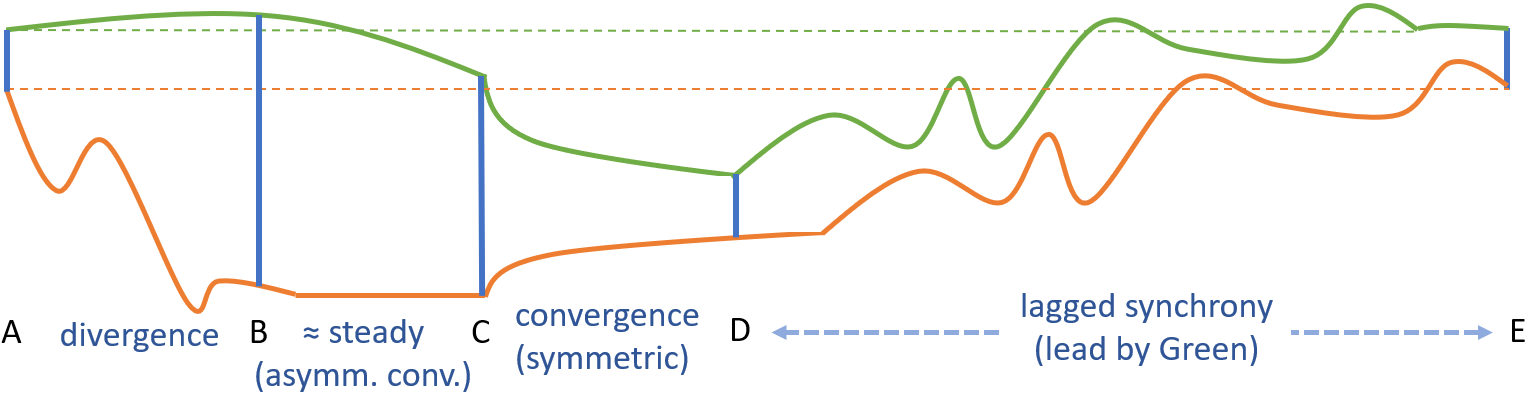
\includegraphics[width=\linewidth]{accommodation_types}
	\caption[Different accommodation types in a conversation]
		{The evolution of a feature's values produced by two speakers represented by the green and orange solid lines.
		The dashed lines connect the corresponding initial and final values of each speaker.
		The letters A to E mark timestamps with behavioral changes.
		Each caption describes the behavior between the two corresponding marks.}
	\label{fig:accommodation_types}
\end{figure}

\section{Pronunciation varieties}
\label{sec:pronunciation_varieties}

\todo[inline]{some introduction...}

\subsection{Long-term and short-term sound changes}
\label{subsec:sound_change}

% use these descriptions in a sentence to describe the nature of the respevtive changes
%\subsection[Long-term sound change]{Sound change as part of a long-term language evolve process}
%\subsection[Short-term phonetic change]{Phonetic change as a short-term social process}

\citet{Ohala1989sound}\\
\citet{Ohala1990phonetics}\\
\citet{Ohala1993phonetics}\\ % this is the main thing
\review{would be cool to have some really old references here. probably there is something in one of Ohala's papers}

\todo[inline]{start with Harrington's paper about the changes in the queen's phonetics over 60 years or so when talking to the people. explain that this is mid-term change, since it's not a change in language, but also not during a single conversation, but rather over a series of "conversations" with the same crowd}

\todo[inline]{here talk (very) long term changes (i.e., not in a single conversation). papers of Ohala (especially 1993 book) are good here, and look for more references from there}

\todo[inline]{transition to short-term changes and say that in this work only this kind of changes are discussed, i.e., within a single conversation or a few chronologically close interactions}

\subsection{Terminology -- variation types}
\label{subsec:variation_types}

The term \enquote{convergence} is a central notion in this work.
This term's definition in this work is different from its meaning in other fields, like \ac{ml}.
Moreover, a wide range terms are used in the literature synonymously to describe the same phenomena, although there are often subtle differences or emphases on specific angles of it.
Disambiguate these various terms should help to avoid confusion and allow more fine-grained description of such processes.
The core meaning of convergence is explained here in details, followed by a list of related terms and explanations about their use in the literature.

The verb \textit{to converge} is defined in Cambridge Dictionary\footnote{\url{http://dictionary.cambridge.org/dictionary/english/converge}} as moving toward, or merging into, the same point (e.g., roads).
A more non-materialistic definition is provided as well: \enquote{If ideas and opinions converge, they gradually become similar}.
Another, somewhat more general, definition to the noun \textit{convergence} is given in Merriam-Webster dictionary\footnote{\url{https://www.merriam-webster.com/dictionary/convergence}}: \enquote{the act of converging and especially moving toward union or uniformity}.
As all these definitions suggest, the core idea of this concept is two (or more) entities that change (potentially in different degrees) toward some physical or abstract point and ultimately meet.
In some time-dependent cases, like spoken interactions, this point can be expected to be withing the range of the entities (the speakers).
Further more, in such cases there might not be enough time for the them to meet, but to become closer, more similar, to one another nonetheless.
This matches the definition of \emph{phonetic convergence} proposed by \citet{Pardo2006phonetic}: \enquote{[\ldots] increase in segmental and suprasegmental similarities between two speakers}.
This also resembles the definition suggested by \citet{Xia2014prosodic}: \enquote{[\ldots] behaviors become more similar over time}, with \enquote{behaviors} referring to different modalities of communications in conversation, e.g., facial expressions, gestures, lexical choices, etc.
\review{make sure the direct quotes are accurate}
Other terms are sometimes used to describe similar processes or different aspects, and it is important to make the distinction between them.
Note that some of the terms are used interchangeably, as synonyms, or as hypernyms and hyponyms in other works.

The list presented here aims to unequivocally distinguish these terms and grant them useful relations to offer a meaningful common terminology, at the very least within the scope of this work and hopefully in the community of this research area in general.

\todo{create/find figures that describe (at least for some)?}
\todo{maybe create a table to compare all of them based on: mutual/one-sided, account for both increase and decrease, has a specific variation as a goal, what aspects is emphasizes (mutuality, initiating the effect, awared or not, capability, etc. maybe group the table by this text-based field and make the others yes/no (with V and X) columns) etc.}
\begin{description}
	\item[accommodation] -- often used as an overarching term, comes from accommodation theory (?). Includes any dynamic (or rather \emph{responsive}, see \putref{ref to accommodation levels}) changes during an interactions.
	Refers to both increase and decrease in similarity.
	
	\item[convergence] -- \ldots
	each speaker can account for a different \enquote{amount} of the convergence.
	it can also be symmetric (examples in Fig 1.1)
	(see illustration in Figure 1 in \citet{Levitan2011measuring})
	[after all sentence about convergence] Similarly, \textbf{divergence}\ldots
	
	\item[assimilation] -- implies a one-sided process, where one side changes in a certain way to match the other.
	It is seen more as a process that occurs as a result of a specific area/context.
	This term is typically used in Phonology to describe changes in pronunciation, e.g., when voiceness of a sound changes to match this of the sound adjacent to it.
	For more details and examples, see \citet[][pp.\ 89-98]{Hall2011phonologie}.
	Note that assimilation is only one of the phonological processes (others would be dissimilation, epenthesis, elision, and more), but since it's the once describing two things becoming more similar to each other, it is the one that might be used in this context.
	
	\item[entrainment] -- is presented by \citet{Brennan1996lexical} as the (potentially aware) influence of an interlocutor on another, e.g., to impose lexical units in an interaction, with emphasis on the on-sided nature of the effect.
	This means that one of the interlocutors established the use of an aforementioned term which created a bias by the conversation partner to employ it as well.
	The change is sometimes seen as categorical (similar to \textit{priming}), which is a key difference from the definition of convergence here.
	This is especially relevant in \ac{hci}, as it is much easier for a computer, due to the vocabulary problem \citep{Furnas1987vocabulary}, to establish such uses.
	\citet{Lopes2013automated} describes entrainment as imposed by a human speaker, where a computer-based interlocutor follows the lexical choices of the user.
	This term is sometimes also used a static measure of changes in an interaction (cf.\ \cref{subsec:limitations_of_did}), as in \citet{Levitan2013entrainment}.
	Conversely, \emph{convergence} is refereed here to the potentially mutual dynamic measure, the difference being comparing discrete timestamps in the interaction (for example, between two halves of a session, as done by \citet{Xia2014prosodic}) versus changes occurring gradually over its entire length.
	In addition to all the above, entrainment is often synonymous to convergence or accommodation in more technical fields.
	
	\item[priming] -- is similar to entrainment, but usually works on a larger scope -- both in terms of change and time.
	As oppose to entrainment, e.g., on the lexical level, priming can influence not just the use of one specific term, but a whole semantic field, and more in psycholinguistics contexts.
	For example, it was shown in experiments \citep[e.g.,][]{Meyer1971facilitation, Schvaneveldt1973retrieval} that people will response faster to words from a specific semantic field after being exposed to other words from it (i.e., different words that are semantically related).
	In more general terms, priming changes the likelihood of a person to use specific behavior, typically on some semantic or syntactic level.
	The temporal scope is different as well.
	Priming can have an effect in a longer term than a single interaction, ranging from multiple interactions, hours, days, and up to years.
	This is why priming is often referred to when talking about children \citep[see, e.g., ][]{Huttenlocher2004syntactic, Wansink2012would}.
	Like entrainment, priming also typically describe categorical change, as oppose to gradual change on a scale (see \textit{entrainment} above and cf.\ \citet{Reitter2006computational, Pace2013concept}).
	
	\item[adaptation] -- refers to the process of making intentional changes that suit certain conditions or situations.
	As such, this term stresses the ambition of these aware modifications in vocal behavior made by an interlocutor to be more similar to another, known and defined, target exhibited by another speaker.
	\citet{Kang2010emergence, Hwang2015phonetic} both examine phonetic adaptation process that occur gradually when encountering a new sound environment, to which speakers want or are expected to adapt.
	In these cases, the changes are also likely to be maintained outside the scope of a specific interaction.
	Adaptation is also used to describe the technical capability -- or more often the lack of one -- in a machine to match its speech production (typically to a user talking with the system).
	This fits the definition of adaptation being intentional and having a well-defined target to adapt towards.
	However, this is still a very limited feature due to the state of \ac{tts} technologies.
	The challenges and integration of such capabilities into \acp{sds} are discussed in \cref{sec:adaptive_spoken_dialogue_systems,chap:convergence_module_for_sdss}.
	
	\item[alignment] -- difference from assimilation? Maybe refers more to the time-aspect, that the interlocutors change in the same times, but not necessarily in the same way? Iona talk a bit about alignment in the introduction of the 2018 journal paper.
	specifically Interactive Alignment Model \citep{Pickering2004behavioral}
	
	\item[synchrony] -- refers to an ongoing process where the interlocutors are changing their behavior similarly, i.e., synchronously.
	Importantly, this applies for the relative change in each speaker, but not to any absolute values.
	That is, the distance is generally maintained while the individual ranges may differ (see Figure 1 in \citet{Levitan2011measuring}).
	When one of the speakers is leading the synchrony, it becomes \emph{lagged}, as shown in \cref{fig:accommodation_types}.
	Lagged phenomena are often identified, and their leader determined, using some correlation measure, like Perason's coefficient in \citet{Edlund2009pause, Xia2014prosodic}.
	A deeper analysis of such accommodation effect is presented in \cref{sec:analysis_hhi}.
	
	\item[mirroring] -- the potentially unaware cognitive effort to produce an output that follows some input.
	A.k.a.\ \enquote{mirrored equivalence} \citep{Messum2015creating, Messum2007mirroring}, this process differs from imitation by the lack of aim toward a well-defined target, but rather an internal representation of the similarity between the speakers.
	This may lead to a less planned and sometimes automatic effect of becoming closer to an interlocutor, where the specifications of the change do not necessarily match the input target.
	Less commonly, this term also refers to an effect opposite to synchrony, where the directions of the respective changes are reversed instead of similar (as if a mirror was put between them).
	Additionally, mirroring may also refer to an effect similar to mimicry, but with greater emphasis on speech learning and acquisition \citep[e.g.,][]{Yoshikawa2003constructivist}.
	
	\item[mimicry] -- is the tendency to behave, or speak, broadly like someone else.
	The emphasize here is on the \emph{general} inclination, which hints it can be done unintentionally, or, alternatively, be deliberate, but without the goal to perfectly match the target (as oppose to imitation).
	% inspired by https://www.voices.com/blog/mimicry_vs_imitation/
	\citet{Gueguen2009mimicry} demonstrate how mimicry can earn the mimicker more favorable judgment in social interactions.
	This is explained by mimicking creating greater feeling of affiliation and rapport in communication, or with the more positive evaluation of the mimicked person due to an enhanced familiarity established by the mimicker.
	\citet{Parrill2006seeing} show just how natural mimicry is in \ac{hhi} in an experiment where participants' behavior was affected merely by watching mimicking takes place in another conversation.
%	reference, mention \textit{Chameleon effect}\ldots
	
	\item[imitation] -- similar to mimicry, but is done awarely and with the goal to match as much closely as possible to a target.
	In addition, emphasizes the speaker's intent to completely match the auditory input \citep[cf.][]{Gueguen2009mimicry}.
	% inspired by https://www.voices.com/blog/mimicry_vs_imitation/
	The attempt to \emph{deliberately} repeat and \emph{accurately} replicate another speaker's productions distinguishes imitation from mirroring and mimicry.
	
	\item[chameleon effect] -- \citep{Chartrand1999chameleon}\\the very beginning of introduction of \citet{Gueguen2009mimicry} also have some good sentences
	
	\item[proximity] -- describes general closeness between interlocutors (as illustrated in Figure 1 in \citet{Levitan2011measuring}).
	This does not imply specific distance thresholds or absolute value ranges.
	Furthermore, this is a rather passive, potentially merely circumstantial, situation, which does not involve a vocal target or an aspiration to match it.
	The proximity at a specific point in time (typically around the start of a conversation) can be used as a reference point for other measures.
	
	\item[coordination] -- implies cooperation -- either seemingly or real -- between the interlocutors, i.e., that there is a common goal to achieve.
	Increase or decrease of communication features is in this case a side of effect of this coordination.
	This provides another point of view on the process, namely not to examine the speakers' collaboration based on common changes, but looking at the changes knowing they are collaborating.
	
	\item[inter-speaker influence] -- a general term to describe a change by a human interlocutor caused by another.
\end{description}

\begin{table}[t]
	\centering
	\caption[Comparison of variation types]
		{Comparison of variation types characteristics.
		[explain each column]
		[explain tick and paranthesesed tick]
		The \enquote*{*} signs mark the terms most frequently used in the literature.}
	\label{tab:variation_types}
	\begin{tabularx}{\linewidth}{Xcccc}
		\toprule
								&	mutuality			&	directionality	&	 intention/awareness	&	well-defined target	\\
		\midrule
		accommodation*			&	\ding{71}			&					&							&						\\
		\rowcolor{lightgray}
		convergence*			&						&					&							&						\\
		assimilation			&						&	\ding{51}		&	\ding{71}				&	\ding{51}			\\
		\rowcolor{lightgray}
		entrainment*			&						&	\ding{51}		&							&	\ding{71}			\\
		priming					&						&	\ding{51}		&	\ding{71}				&	\ding{51}			\\
		\rowcolor{lightgray}
		adaptation*				&						&	\ding{51}		&	\ding{51}				&	\ding{51}			\\
		alignment				&						&	\ding{51}		&	\ding{71}				&	\ding{51}			\\
		\rowcolor{lightgray}
		synchrony				&	(\ding{51})			&	\ding{71}		&							&						\\
		mimicry					&						&	\ding{51}		&	\ding{71}				&	\ding{51}			\\
		\rowcolor{lightgray}
		imitation				&						&	\ding{51}		&	\ding{51}				&	\ding{51}			\\
		mirroring				&						&	\ding{51}		&	\ding{51}				&	\ding{51}			\\
		\rowcolor{lightgray}
		chameleon eff.			&	?					&		?			&			?				&		?				\\
		proximity				&						&					&							&						\\			
		\rowcolor{lightgray}
		coordination			&	\ding{51}			&					&	\ding{51}				&	\ding{71}			\\
		int.sp. influence		&						&	\ding{51}		&	\ding{71}				&	\ding{71}			\\
		\bottomrule
	\end{tabularx}
\end{table}

\section{Vocal accommodation in human-computer interaction}
\label{sec:phonetic_convergence_in_hci}

% lettrine text: Paradigms and interfaces of human interaction with machines are described in this chapter, with emphasis on more modern forms of interaction with computers and mobile devices.
%The importance, advantages, and challenges of verbal interaction are discussed here as well.

%\subsection{What is an interaction?}
%\label{subsec:what_is_an_interaction}

\subsection{Verbal interaction with computers}
\label{subsec:verbal_interaction}

In \ac{hhi}, an \emph{interaction} is a mutual or reciprocal relationship between two (or more) interlocutors within a defined timespan.
This is also true for interaction with machine, though the beneficial side is typically the human speaker(s) while the machine is used to achieve the humans' goal.
In more modern application, and especially when \ac{ai} is involved, the computer might also be programmed to \enquote{benefit} from the interaction, e.g., by acquiring information for future interactions or being able to finish a task more efficiently.
One type of interaction is a \emph{conversation}, where the communication is language-based.
This difference is more prominent in \ac{hci}, since there are ways to interact with machines without using written or spoken words, like using touchscreens, a computer mouse, or hand gestures. This can be compared to non-verbal -- neither written nor spoken -- human communication, but purely non-verbal communication occurs more often with machines than with people.
The main reason for that is probably since machines are not, yet, capable of using language as freely and verbosely as humans.
The terms \enquote{interaction} and \enquote{conversation} are often used interchangeably in this work, since the interaction in question are spoken conversations.
Nevertheless, interactions refer to more general concept of communication that might involve other components than speech and conversations focus on the language components of the communication.
% spoken interaction -- Although the linguistic content might remain the same, adds complexity due to variety or speech and the technological challenge of generating inteligble speech output.

Interestingly, humans almost always need to compromise on the way they interact with computers, or learn new interfaces (like those mentioned above) even for performing simple tasks.
Even in the case of spoken communication, which develops early on in humans, compromises need to be made as to how to speak to the computer so that it understands that user's intention.
For any of the system types mentioned in \cref{sec:types_of_sdss}, users needs to learn how to modify their speech so that they can properly use the systems (be it the speech style of wording), instead of the system being able to adapt to the user.
With the advance of speech technology, this gap is shrinking, but there is still a way to go before computers will be able to understand and produce spoken language well enough that people are able to speech to computers as they speak to other human-beings.
The topics of this work capitalizes on this evolution, to see whether \ac{hhi} phenomena like vocal accommodation are transferred to \ac{hci} as talking to computers becomes easier and more common.
More generally, the question rises whether \ac{cat} holds for \ac{hci} as well.
This is supported, for example, by the \ac{casa} paradigm \citep{Nass2000machines}, which argues that humans apply similar social behaviors when interacting with computers because they ascribe human characteristics to them.
As a starting point, domain-specific systems with alternate turn taking are easier for computers, as they take away a lot of the complexity of spoken language and reduce it to individual utterances that can be mapped to actions the system supports.
For example, a \ac{sds} for ordering train tickets will probably follow a very specific protocol and react only to specific input, as opposed, for example, for a general-purpose system that could talk with the user about a planned trip and help booking tickets as part of a longer, general-purpose conversation (see \cref{tab:sds_types}).

\subsection{Previous work}
\label{subsec:previous_work}

\todo{maybe there is a better title for this section?}

\Cref{subsec:linguistic_accommodation} discusses vocal accommodation in \ac{hhi}, but this phenomenon has been studied in \ac{hci} as well.
A key difference between the two settings is the lack of naturalness on the computer's side. 
Since accommodation is often ascribed to mutual social aspects (as explained by \ac{cat} in \cref{sec:communication_accommodation_theory}), this introduces a limitation in the amount of accommodation that may occur.
Two main approaches are used to overcome this limitation in experiments:
Simulating a computer's output in a wizard-of-Oz setting and integrating some accommodation capabilities into a \ac{sds}.
Wizard-of-Oz experiments have the advantage that the output of the computer-based interlocutor can be directly controlled by the experimenter, usually using pre-defined utterances.
This grants precision and control over the experiment, which makes it a very suitable approach for research.
However, preparing the experimenter's control interface and the utterances might be time consuming, e.g., if they need to be recorded or manually manipulated in a certain way.
Another disadvantage is the disability to deviate from a pre-defined script covered by the prepared utterances, limiting the variety of interactions the simulated system can support.
\Acp{sds} that support at least some level of accommodation or real-time manipulation save the time and effort of creating stimuli prior to the experiment.
Though the quality of the output and the time required to generate it might be affected, this setting better represents real-world \ac{hci} and can typically better react to varying paths the experiment is going (depending on its domain constraints).
As with real-world systems, it requires a lot of time to develop these capabilities, which often makes this option impractical in research.
\Cref{sec:adaptive_spoken_dialogue_systems} discusses further facets and possible solutions for integrating accommodation capabilities into \acp{sds}.

Using these two methods, various experiment have been conducted to measure accommodation in \ac{hci}.
%Various studies have investigated entrainment and priming in \acp{sds}, aiming to better understand \ac{hci} dynamics and improve task-completion rates.
\citet{Bergqvist2020nontrivial, Lopes2011primes}, for example, focused on dynamic entrainment and adaptation on the lexical level, and found users adapt to a system's terminology that differs from theirs.
This also led to improved performance in the given tasks.
\citet{Parent2010lexical} examined correlation of lexical choices and word frequency using the \emph{Let's Go}~\ac{sds} \citep{Raux2005letsgo} and found that users adapt more to words that occur more often.
While these studies addressed the changes in experimental, scripted scenarios, the theoretical foundations for studying these changes in spontaneous dialogue exist as well \citep{Brennan1996lexical}.
\citet{Gasic2013policy, Levin2000stochastic} provide examples of online adaptation for dialogue policies and strategies.
Noticeably, while all of the studies mentioned above examine various facets of dialogues, none of those are related to the auditory aspects of speech -- the primary modality used to interact with \acp{sds}.
\citet{Benus2018prosodic} found relationships between the level of user's trust toward an avatar and the degree of the system's vocal entrainment or disentrainment.
Similarly, \citet[][pp.\ 142-144]{Levitan2014acoustic} shows relationships between prosodic entrainment and how much participants liked the avatar they were interacting with.
\citet{Bell2003prosodic} found that users' speech rate can be manipulated using a human-simulated \ac{sds}.
Similar results were found when intensity changes in children's interaction with synthesized output were examined \citep{Coulston2002amplitude}.
All these experiments focus on \ac{hci}, while those in \cref{subsec:linguistic_accommodation} concentrate on \ac{hhi}.
However, accommodation in \ac{hhi} and \ac{hci} has not been directly compared within the same interaction, as done in \cref{chap:speech_variations_in_hhci}.
Furthermore, mainly suprasegmental characteristics have been studied for accommodation in \ac{hci}, mostly due to technical limitations (see \cref{sec:adaptive_spoken_dialogue_systems} for details).
a wizard-of-Oz experiment with focus on \emph{segmental} features is described in \cref{chap:shadowing_experiment_with_natural_and_synthetic_voices}.